
\section{Theoretical Analysis}
\label{sec:analysis}
\vspace{3mm}
\par In this section, the previously shown circuit is theoretically analised.
\vspace{3mm}
\par
The considered circuit is divided in a gain and an output stages. In the gain stage, the transistor $Q_1$ is operating in the forward active region, and the capacitor $C_1$ blocks the DC component of $V_{in}$, causing an open circuit at low frequencies. In sum, the bias circuit $V_{CC},R_1,R_2$ will ensure the BEJ is ON.
\par The output stage is responsible for lowering the output impedance so that there is compatibility with the $8\Omega$ speaker (load).


\par The circuit was analyzed by operating point. Therefore, it is possible to compute values such as the Input Impedance, Output Impedance and Gain, separately for both stages and for the total circuit.We can separate the stages and later connect their values \textbf{without significant loss} because, when comparing the impedance of both stages, one notices that the second stage (output stage) has a much greater impedance than the first one (gain). Hence, a considerably part of the voltage will be dropped in the output stage. Also, it is legit to think that the low impedance value is in harmony with the $8\Omega$ value for the load impedance. It was also possible to reach some values to be used in the incremental model for the transistor ($r_{\pi}$ ; $r_O$ ; $g_m$). The following figure presents precisely the considered incremental model for the transistor:

\begin{figure}[h] \centering
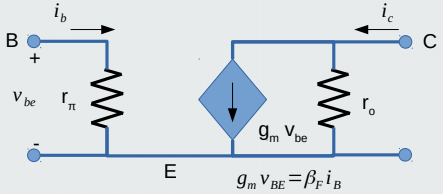
\includegraphics[scale=0.5]{incre.png}
\caption{Incremental model for transistors.}
\label{incretrans}
\end{figure}

\par The resulting values are all presented ahead, side by side with the ones obtained via simulation, for the purpose of comparison.

\par Finally, the frequency response of the circuit was studied, from where the gain $\frac{V_{out}(f)}{V_{in}(f)}$ was obtained, by means of the nodal method, applied with the transistor incremental model, resulting in the following system (with $G_x=\frac{1}{R_x}$ and $g_{\pi_x}=\frac{1}{r_{\pi_x}}$):

\begin{center}
  $\begin{cases} (V_{in2}-V_{in})G_{in}+(V_{in2}-V_{base})j \omega C_i=0  \\ V_{base}G_2 + (V_{base}-V_{CC})G_1 + (V_{base}-V_{in2})j \omega C_1 + (V_{base}-V_{emit})g_{\pi_1}=0 \\ V_{emit}G_E + V_{emit}j \omega C_b + (V_{emit}-V_{base})g_{\pi_1}+(V_{emit}-V_{coll})g_{O_1}-(V_{base}-V_{emit})g_{m_1}=0 \\ (V_{coll}-V_{CC})G_C + (V_{coll}-V_{emit})g_{O_1}+(V_{base}-V_{emit})g_{m_1}+(V_{coll}-V_{emit2})g_{\pi_2}=0 \\ (V_{emit2}-V_{CC})G_{out} + (V_{emit2}-V_{out})j \omega C_O + (V_{emit2}-V_{coll})g_{\pi_2} + V_{emit2}g_{O_2}-(V_{coll}-V_{emit2})g_{m_2} =0 \\ V_{out}G_L + (V_{out}-V_{emit2})j \omega C_O =0  \end{cases}$
\end{center}


\par Again, the plot result is presented side by side with the simulation one, ahead.
%\vspace{100mm}
